% =====================================================================
%  Graph Neural Networks --- MiRA Training Course 2026
%  Speaker: 仲翊 | 9/3, 17:20-17:50, R546 | 30 minutes
%
%  COMPILE (XeTeX-based engine required: the deck uses fontspec + a CJK font)
%      tectonic gnn_talk.tex            <- verified working
%      xelatex gnn_talk.tex             (twice, if tectonic is unavailable)
%      ./compile.sh gnn_talk.tex
%
%  SPEAKER NOTES: uncomment the \setbeameroption line below to print them.
% =====================================================================
\documentclass[aspectratio=169,11pt]{beamer}

% ---- theme -----------------------------------------------------------
\usetheme{metropolis}
\metroset{progressbar=frametitle, sectionpage=none, numbering=none}

% ---- fonts (XeLaTeX/LuaLaTeX + fontspec; CJK for the speaker's name) --
\usepackage{fontspec}
\newfontfamily\cjkfont{Noto Sans CJK TC}[Scale=MatchLowercase]
\newcommand{\CJK}[1]{{\cjkfont #1}}
% If "Noto Sans CJK TC" is missing on the build machine, swap the family
% above for any installed CJK face (for example "Noto Sans CJK SC" or "WenQuanYi Zen Hei").

% ---- packages --------------------------------------------------------
\usepackage{booktabs}
\usepackage{array}
\usepackage{amsmath, amssymb}
\usepackage{tikz}
\usetikzlibrary{arrows.meta, positioning, calc, backgrounds, fit}
\usepackage{listings}
\usepackage{xcolor}

% ---- colours ---------------------------------------------------------
\definecolor{acc}{HTML}{C0392B}      % accent: the piece under discussion
\definecolor{acc2}{HTML}{2C7BB6}     % secondary accent
\definecolor{dim}{HTML}{AAAAAA}      % greyed-out
\definecolor{good}{HTML}{1B7837}
\setbeamercolor{alerted text}{fg=acc}

% ---- code listings ---------------------------------------------------
\lstset{
  basicstyle=\ttfamily\small,
  keywordstyle=\color{acc2}\bfseries,
  commentstyle=\color{dim}\itshape,
  stringstyle=\color{good},
  language=Python,
  showstringspaces=false,
  columns=fullflexible,
  breaklines=true,
  frame=none,
  aboveskip=0.4em, belowskip=0.4em,
}

% ---- speaker notes ---------------------------------------------------
% \setbeameroption{show notes}                    % <- uncomment to print notes
% \setbeameroption{show notes on second screen=right}

% ---- shorthands ------------------------------------------------------
\newcommand{\arx}[1]{{\scriptsize\color{dim}arXiv:#1}}
\newcommand{\hv}{h_v}
\newcommand{\hu}{h_u}
\newcommand{\Nv}{\mathcal{N}(v)}

% =====================================================================
\title{Graph Neural Networks}

\author{\CJK{仲翊}}
\date{MiRA Training Course 2026 \quad$\cdot$\quad 9/3, R546}
% =====================================================================

\begin{document}

% --- 1 ----------------------------------------------------------------
\begin{frame}[plain]
  \titlepage
\end{frame}
\note{Last talk of an 8.5-hour day. Say the time promise in your first sentence.
Skip the warm-up. Target: finish at 17:48.

CHECKPOINT: 17:20 here.}

% --- 2 ----------------------------------------------------------------
\begin{frame}{Three properties of graph neural networks}
  \begin{enumerate}
    \setlength{\itemsep}{1.1em}
    \item Each node makes a \alert{summary of its neighbors}, then updates itself.
    \item Each layer extends the view of a node by \alert{one hop}. Two or three
          layers is the usual optimum.
    \item \alert{Graph construction} decides how a GNN performs. The layer
          architecture matters less.
  \end{enumerate}
\end{frame}
\note{Say the promise aloud: "30 minutes, 3 ideas, I stop at 17:50." Tell them
there is one equation and no spectral graph theory. Then stop early.

Do not define a graph yet. Show four robot pictures first.}

% --- 3 ----------------------------------------------------------------
\begin{frame}{Outline}
  \tableofcontents
\end{frame}

% =========================================================================
\section{What GNNs are for}
% =========================================================================

% --- 3 ----------------------------------------------------------------
\begin{frame}{Three task types, three readouts}
  \vspace{0.8em}
  \begin{itemize}
    \setlength{\itemsep}{1.1em}
    \item \textbf{Node-level}: the prediction is $h_v$.\\
      {\small Label each point in the cloud. Predict the next position of each particle.}
    \item \textbf{Edge-level}: the prediction is a function of $(h_u, h_v)$.\\
      {\small Will this pair collide? Is this a loop closure?}
    \item \textbf{Graph-level}: a \alert{readout} sums or averages all nodes,
      then an MLP predicts.\\
      {\small Is this scene graspable? Will this grasp succeed?}
  \end{itemize}
\end{frame}
\note{Tell them to pick the row that fits their own project before they pick
an architecture. Do not take
answers. There is no time.}


% --- 4 ----------------------------------------------------------------
\begin{frame}{What the nodes and edges were}
  \vspace{-0.5em}
  \centering
  \scriptsize
  \setlength{\tabcolsep}{4pt}
  \renewcommand{\arraystretch}{1.0}
  \begin{tabular}{@{}>{\raggedright\arraybackslash}p{3.15cm}
                    >{\raggedright\arraybackslash}p{2.50cm}
                    >{\raggedright\arraybackslash}p{2.95cm}
                    >{\raggedright\arraybackslash}p{4.10cm}@{}}
    \toprule
    \textbf{Application} & \textbf{Nodes} & \textbf{Edges} & \textbf{Paper} \\
    \midrule
    Multi-arm motion planning & arms, tasks, obstacles & possible collisions
      & RoboBallet \arx{2509.05397} \\
    Deformables and fluids & particles of the object & contact + rigid-group
      & DPI-Net \arx{1810.01566} \\
    Learned physics & particles & within a radius
      & GNS \arx{2002.09405} \\
    Learned physics (mesh) & mesh vertices & mesh edges
      & MeshGraphNets \arx{2010.03409} \\
    Deformables from vision & object keypoints & learned latent graph
      & \arx{2104.12149} \\
    Point clouds & points & k-NN, recomputed \emph{in feature space}
      & DGCNN / EdgeConv \arx{1801.07829} \\
    Grasp pose detection & points of the cloud & local neighborhoods
      & Grasp-the-Graph 2.0 \arx{2505.02664} \\
    Multi-robot planning & robots & communication range (decentralized)
      & Li \& Prorok \arx{1912.06095} \\
    Spatial perception & places, objects, agents & containment, adjacency
      & 3D Dynamic Scene Graphs\newline\arx{2002.06289} \\
    \bottomrule
  \end{tabular}
  \vspace{0.5em}

  \footnotesize
  \alert{In every row, the edges encode a physical relation that the authors
  knew before training.}
\end{frame}
\note{Tell them to copy the Nodes and Edges columns into their own project.
Do not read the table. Point at two rows. The first is DGCNN, which
recomputes the edges in feature space and surprises people. The second is the
row closest to the projects in this room.

Tell them that the slide is in the repo, so they do not photograph it.}


% =========================================================================
\section{The message-passing layer}
% =========================================================================

% --- 5 ----------------------------------------------------------------
\begin{frame}{Message passing: aggregate neighbors, update, repeat}
  \vspace{-0.4em}
  \begin{center}
    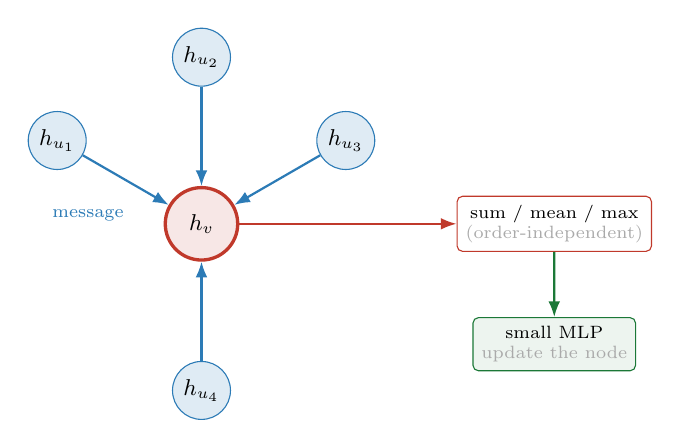
\begin{tikzpicture}[scale=0.92, every node/.style={transform shape},
      nb/.style={circle, draw=acc2, fill=acc2!15, minimum size=8mm,
                 font=\small, inner sep=0pt},
      me/.style={circle, draw=acc, very thick, fill=acc!12, minimum size=10mm,
                 font=\small, inner sep=0pt},
      msg/.style={-{Latex[length=2mm]}, acc2, thick}]

      \node[me] (v) at (0,0) {$\hv$};
      \node[nb] (u1) at (150:2.3) {$h_{u_1}$};
      \node[nb] (u2) at ( 90:2.3) {$h_{u_2}$};
      \node[nb] (u3) at ( 30:2.3) {$h_{u_3}$};
      \node[nb] (u4) at (270:2.3) {$h_{u_4}$};

      \foreach \u in {u1,u2,u3,u4} \draw[msg] (\u) -- (v);
      \node[color=acc2, font=\scriptsize, anchor=north east] at (-0.95,0.32)
        {message};

      \node<2->[draw=acc, fill=white, rounded corners=2pt, font=\scriptsize,
            right=3.0cm of v, align=center] (agg)
        {sum / mean / max\\ \color{dim}(order-independent)};
      \draw<2->[-{Latex[length=2mm]}, acc, thick] (v) -- (agg);

      \node<3->[draw=good, fill=good!8, rounded corners=2pt, font=\scriptsize,
            below=0.9cm of agg, align=center] (upd)
        {small MLP\\ \color{dim}update the node};
      \draw<3->[-{Latex[length=2mm]}, good, thick] (agg) -- (upd);
    \end{tikzpicture}
  \end{center}
  \vspace{-0.3em}
  \begin{enumerate}
    \item<1-> Each neighbor \alert{sends a message}.
    \item<2-> The node combines them with an \alert{order-independent} function: sum, mean or max.
    \item<3-> The node \alert{updates its own vector} with a small MLP. The layer repeats $L$ times.
  \end{enumerate}
\end{frame}
\note{Say the sentence before any notation appears. Do not rush this slide, and
do not add symbols yet. If they remember one slide, make it this one.}

% --- 6 ----------------------------------------------------------------
\begin{frame}{The message-passing equation: MSG, AGG, UPDATE}
  \vspace{1.6em}
  \begin{center}
    \large
    \only<1>{$\hv \;\leftarrow\; \textcolor{dim}{\mathrm{UPDATE}\Big(\hv,\;
      \mathrm{AGG}\big\{}\;\textcolor{acc}{\mathrm{MSG}(\hv, \hu, e_{uv})}\;
      \textcolor{dim}{:\; u \in \Nv \big\}\Big)}$}
    \only<2>{$\hv \;\leftarrow\; \textcolor{dim}{\mathrm{UPDATE}\Big(\hv,\;}
      \textcolor{acc}{\mathrm{AGG}\big\{}\;\mathrm{MSG}(\hv, \hu, e_{uv})\;
      \textcolor{acc}{:\; u \in \Nv \big\}}\textcolor{dim}{\Big)}$}
    \only<3->{$\hv \;\leftarrow\; \textcolor{acc}{\mathrm{UPDATE}\Big(}\hv
      \textcolor{acc}{,}\;
      \mathrm{AGG}\big\{\;\mathrm{MSG}(\hv, \hu, e_{uv})\;:\; u \in \Nv \big\}
      \textcolor{acc}{\Big)}$}
  \end{center}
  \vspace{1.8em}
  \begin{center}
    \only<1>{\alert{A neighbor $u$ sends a message to $v$.} The message can use
      the features of $v$, the features of $u$, and \emph{the edge feature $e_{uv}$}.}
    \only<2>{\alert{AGG combines all the messages} with a sum, mean or max.
      Because that function ignores order, the layer is permutation invariant.}
    \only<3>{\alert{UPDATE is a small MLP} on $(h_v,\ \text{summary})$.
      That completes one layer.}
    \only<4>{\alert{A GNN is $L$ of these layers}, stacked.}
  \end{center}
  \vspace{1.2em}
  \onslide<4->{\begin{center}\small\color{dim}
    GCN in one line: $H \leftarrow \hat{A}\,(H W)$, with
    $\hat{A} = D^{-1/2}(A+I)D^{-1/2}$, a normalized neighbor average, then a
    linear map.
  \end{center}}
\end{frame}
\note{This is the only equation in the talk. Read it left to right, out loud,
one click at a time. Point at the colored piece each time.

Emphasize: $e_{uv}$ is the edge feature. In robotics that is the
relative pose. That design decision is worth more than the architecture.

CHECKPOINT: 17:32 by the end of this slide.}

% --- 7 ----------------------------------------------------------------
\begin{frame}{$L$ layers $=$ an $L$-hop receptive field}
  \vspace{0.2em}
  \begin{center}
    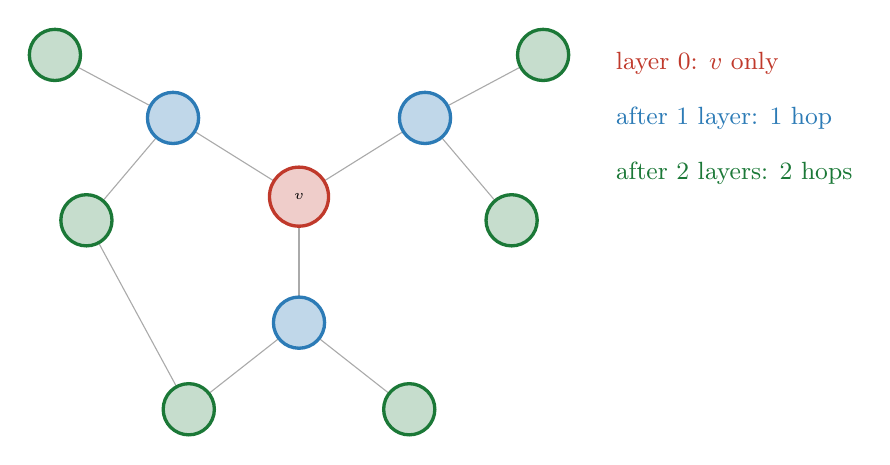
\begin{tikzpicture}[scale=1.0, every node/.style={transform shape},
      n/.style={circle, draw=dim, fill=black!3, minimum size=6.5mm, inner sep=0pt},
      h1/.style={circle, draw=acc2, very thick, fill=acc2!30, minimum size=6.5mm,
                 inner sep=0pt},
      h2/.style={circle, draw=good, very thick, fill=good!25, minimum size=6.5mm,
                 inner sep=0pt},
      me/.style={circle, draw=acc, very thick, fill=acc!25, minimum size=7.5mm,
                 inner sep=0pt}]

      \coordinate (cv) at (0,0);
      \coordinate (ca) at (-1.6, 1.0);  \coordinate (cb) at (1.6, 1.0);
      \coordinate (cc) at (0,-1.6);
      \coordinate (cd) at (-3.1, 1.8);  \coordinate (ce) at (-2.7,-0.3);
      \coordinate (cf) at ( 3.1, 1.8);  \coordinate (cg) at ( 2.7,-0.3);
      \coordinate (ch) at (-1.4,-2.7);  \coordinate (ci) at ( 1.4,-2.7);

      \foreach \x/\y in {cv/ca, cv/cb, cv/cc, ca/cd, ca/ce, cb/cf, cb/cg,
                         cc/ch, cc/ci, ce/ch}
        \draw[dim] (\x) -- (\y);

      % base state: every node grey
      \foreach \c in {ca,cb,cc,cd,ce,cf,cg,ch,ci} \node[n] at (\c) {};
      % 1-hop lights up on click 2
      \node<2->[h1] at (ca) {}; \node<2->[h1] at (cb) {}; \node<2->[h1] at (cc) {};
      % 2-hop lights up on click 3
      \node<3->[h2] at (cd) {}; \node<3->[h2] at (ce) {}; \node<3->[h2] at (cf) {};
      \node<3->[h2] at (cg) {}; \node<3->[h2] at (ch) {}; \node<3->[h2] at (ci) {};
      \node[me] at (cv) {\tiny $v$};

      \node[font=\small, anchor=west, color=acc]  at (3.9,1.70)
        {layer 0: $v$ only};
      \node<2->[font=\small, anchor=west, color=acc2] at (3.9,1.00)
        {after 1 layer: 1 hop};
      \node<3->[font=\small, anchor=west, color=good] at (3.9,0.30)
        {after 2 layers: 2 hops};
    \end{tikzpicture}
  \end{center}
  \vspace{-0.6em}
  \onslide<4->{\begin{center}\large
    After $L$ layers, $h_v$ depends on every node within $L$ hops,\\
    the same way a CNN receptive field grows by one pixel per layer.
  \end{center}}
\end{frame}
\note{To show this live: put a 1 on node 0 and propagate. The non-zero set
grows one hop per layer.

Most of the room already has the CNN receptive-field picture. Give them
the mapping and stop.}



% --- 8 ----------------------------------------------------------------
\begin{frame}{PyTorch Geometric tutorials on Colab}
  \vspace{0.2em}
  \begin{center}\small
    \textbf{Notebooks with cached results}
    \quad{\scriptsize\texttt{github.com/Chung-I/MiRA\_training\_course\_2026/tree/main/notebooks}}
  \end{center}
  \vspace{0.3em}
  \centering\small
  \begin{tabular}{@{}llrl@{}}
    \toprule
    \textbf{Notebook} & \textbf{Dataset} & \textbf{Result} & \textbf{Graph} \\
    \midrule
    \href{https://colab.research.google.com/github/Chung-I/MiRA_training_course_2026/blob/main/notebooks/pyg_node_classification.ipynb}{Node classif.}
      & Cora (2,708 nodes)
      & \textcolor{good}{\textbf{80.7\%}}
      & citation \\
      & {\color{dim}MLP baseline}
      & {\color{dim}54.7\%}
      & {\color{dim}(no graph)} \\[0.3em]
    \href{https://colab.research.google.com/github/Chung-I/MiRA_training_course_2026/blob/main/notebooks/pyg_graph_classification.ipynb}{Graph classif.}
      & MUTAG (188 graphs)
      & 70.5\%
      & molecular bonds \\
    \bottomrule
  \end{tabular}
  \vspace{0.4em}

  \begin{center}\small
    The 26-point gap between MLP (54.7\%) and GCN (80.7\%) on Cora comes
    from the citation graph. The node features alone do not separate the
    classes. The node-classification notebook also contains a layer sweep
    that shows over-smoothing (appendix).
  \end{center}
\end{frame}
\note{Both notebooks are in the repo with cached outputs. Open them in Colab
via the badge at the top of each notebook. Results are visible without
re-running.

The node-classification notebook includes a layer sweep (Section 5) showing
over-smoothing: accuracy peaks at 2 layers (80.7\%) and drops to 61.6\% at 8.

If time allows, open the node-classification notebook and change num\_layers
live. Budget 2 minutes. If a cell fails, close it and point at this slide.

CHECKPOINT: back on slides by 17:44.}


% =========================================================================
\section{GNNs and Transformers}
% =========================================================================

% --- 9 ----------------------------------------------------------------
\begin{frame}{CNN, Transformer, GNN: three structural assumptions}
  \vspace{0.2em}
  \begin{center}
    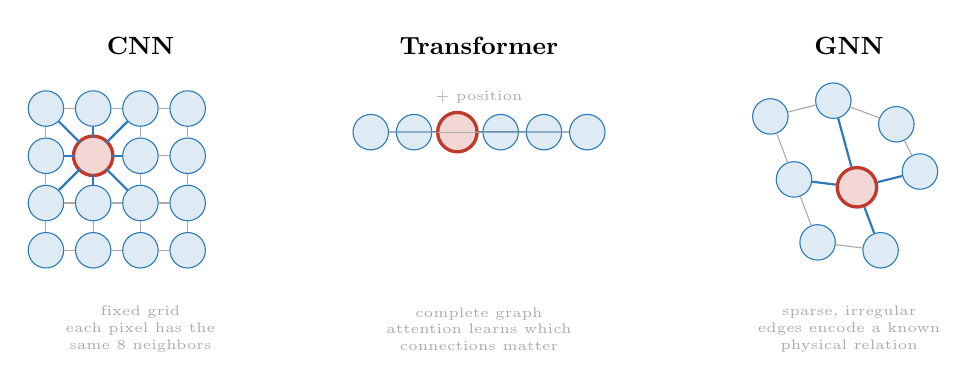
\begin{tikzpicture}[
      font=\scriptsize,
      nd/.style={circle, draw=acc2, fill=acc2!15, minimum size=4.5mm,
                 inner sep=0pt},
      hl/.style={circle, draw=acc, very thick, fill=acc!20, minimum size=5mm,
                 inner sep=0pt},
      ed/.style={dim, line width=0.4pt},
      edc/.style={acc2, line width=0.5pt},
    ]

    % === CNN: 4x4 grid, center pixel highlighted with 3x3 kernel ===
    \node[font=\small\bfseries] at (1.2, 3.6) {CNN};
    \foreach \r in {0,...,3} {
      \foreach \c in {0,...,3} {
        \pgfmathtruncatemacro{\idx}{\r*4+\c}
        \node[nd] (g\idx) at (\c*0.6, 2.8-\r*0.6) {};
      }
    }
    % grid edges (horizontal)
    \foreach \r in {0,...,3} {
      \foreach \c in {0,...,2} {
        \pgfmathtruncatemacro{\a}{\r*4+\c}
        \pgfmathtruncatemacro{\b}{\r*4+\c+1}
        \draw[ed] (g\a)--(g\b);
      }
    }
    % grid edges (vertical)
    \foreach \r in {0,...,2} {
      \foreach \c in {0,...,3} {
        \pgfmathtruncatemacro{\a}{\r*4+\c}
        \pgfmathtruncatemacro{\b}{(\r+1)*4+\c}
        \draw[ed] (g\a)--(g\b);
      }
    }
    % highlight center pixel and its 3x3 neighborhood
    \node[hl] at (1*0.6, 2.8-1*0.6) {};
    \foreach \dr/\dc in {-1/-1,-1/0,-1/1,0/-1,0/1,1/-1,1/0,1/1} {
      \pgfmathtruncatemacro{\nr}{1+\dr}
      \pgfmathtruncatemacro{\nc}{1+\dc}
      \pgfmathtruncatemacro{\ni}{\nr*4+\nc}
      \draw[edc, thick] (g5)--(g\ni);
    }
    \node[font=\tiny, color=dim, align=center] at (1.2, 0.0)
      {\alert{fixed grid}\\each pixel has the\\same 8 neighbors};

    % === Transformer: 6 tokens, fully connected ===
    \node[font=\small\bfseries] at (5.5, 3.6) {Transformer};
    \foreach \i in {0,...,5}
      \node[nd] (t\i) at (5.5+\i*0.55-1.375, 2.5) {};
    % positional encoding arrow
    \node[font=\tiny, color=dim] at (5.5, 2.95) {$+$ position};
    % full connections from token 2
    \node[hl] (t2h) at (5.5+2*0.55-1.375, 2.5) {};
    \foreach \j in {0,1,3,4,5}
      \draw[edc, thick, opacity=0.5] (t2h)--(t\j);
    % all-to-all dim
    \foreach \i in {0,...,5} {
      \foreach \j in {\i,...,5} {
        \ifnum\i<\j
          \pgfmathtruncatemacro{\skip}{(\i==2)||(\j==2)?1:0}
          \ifnum\skip=0
            \draw[ed, opacity=0.3] (t\i)--(t\j);
          \fi
        \fi
      }
    }
    \node[font=\tiny, color=dim, align=center] at (5.5, 0.0)
      {\alert{complete graph}\\attention learns which\\connections matter};

    % === GNN: irregular graph ===
    \node[font=\small\bfseries] at (10.2, 3.6) {GNN};
    \node[nd] (n0) at (9.2, 2.7) {};
    \node[nd] (n1) at (10.0, 2.9) {};
    \node[nd] (n2) at (10.8, 2.6) {};
    \node[nd] (n3) at (9.5, 1.9) {};
    \node[hl] (n4) at (10.3, 1.8) {};
    \node[nd] (n5) at (11.1, 2.0) {};
    \node[nd] (n6) at (9.8, 1.1) {};
    \node[nd] (n7) at (10.6, 1.0) {};
    \draw[ed] (n0)--(n1); \draw[ed] (n1)--(n2); \draw[ed] (n2)--(n5);
    \draw[ed] (n0)--(n3); \draw[ed] (n3)--(n6); \draw[ed] (n6)--(n7);
    \draw[edc, thick] (n4)--(n3); \draw[edc, thick] (n4)--(n5);
    \draw[edc, thick] (n4)--(n7); \draw[edc, thick] (n4)--(n1);
    \node[font=\tiny, color=dim, align=center] at (10.2, 0.0)
      {\alert{sparse, irregular}\\edges encode a known\\physical relation};

    \end{tikzpicture}
  \end{center}
  \vspace{0.2em}
  \begin{center}\small
    A CNN applies a fixed kernel to a regular grid. A Transformer attends
    to all tokens and learns the edge weights. A GNN aggregates over a
    \alert{sparse, problem-specific graph} that the designer provides.
  \end{center}
\end{frame}
\note{The three diagrams make the structural assumption visible. Point at the
highlighted node in each diagram: it has 8 fixed neighbors (CNN), all other
tokens (Transformer), or a sparse set of known neighbors (GNN).

The Distill ``A Gentle Introduction to Graph Neural Networks'' (2021) uses a
similar pixel-grid-to-graph progression. CS224W Lecture 3 has a ``GNNs subsume
CNNs'' section with the same idea.

Ask the room which architecture fits a collision graph or a particle system.
The answer is the rightmost diagram.}

% --- 10 ---------------------------------------------------------------
\begin{frame}{A GNN produces the same output regardless of node ordering}
  \vspace{0.4em}
  \begin{center}
    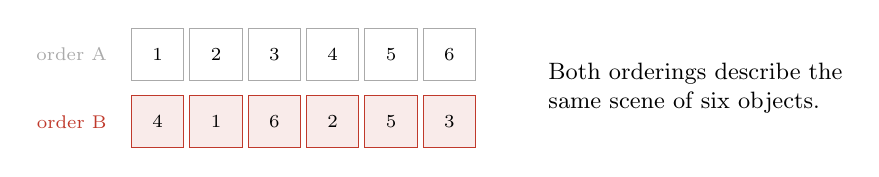
\begin{tikzpicture}[scale=0.95, every node/.style={transform shape},
      box/.style={rectangle, draw=dim, minimum width=7mm, minimum height=7mm,
                  font=\scriptsize}]
      \foreach \i/\lab in {0/1,1/2,2/3,3/4,4/5,5/6}
        \node[box] at (\i*0.78, 0.9) {\lab};
      \node[font=\scriptsize, color=dim] at (-1.15,0.9) {order A};
      \foreach \i/\lab in {0/4,1/1,2/6,3/2,4/5,5/3}
        \node[box, fill=acc!10, draw=acc] at (\i*0.78, 0) {\lab};
      \node[font=\scriptsize, color=acc] at (-1.15,0) {order B};
      \node[align=left, font=\small, anchor=west] at (5.1,0.45)
        {Both orderings describe the\\ same scene of six objects.};
    \end{tikzpicture}
  \end{center}
  \vspace{0.6em}
  A GNN aggregates neighbors with a sum, mean, or max. Because these
  functions \alert{ignore the order of their inputs}, the output is the same
  for any permutation of the nodes. This property is called
  \alert{permutation invariance} (for graph-level predictions) or
  \alert{permutation equivariance} (for node-level predictions, where the
  output permutes with the input).
\end{frame}
\note{Permutation invariance: $f(\pi(G)) = f(G)$ for graph-level output.
Permutation equivariance: $f(\pi(G)) = \pi(f(G))$ for node-level output, meaning
each node's output follows that node's identity, not its position in the vector.

The PyG Introduction tutorial demonstrates this: renumber the nodes and the
GCN output stays the same, while an MLP output changes.}

% --- 11 ---------------------------------------------------------------
\begin{frame}{A GNN accepts a variable number of nodes and edges}
  \vspace{0.2em}
  \begin{columns}[c]
    \begin{column}{0.42\textwidth}
      \centering
      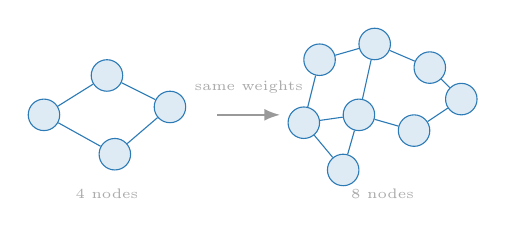
\begin{tikzpicture}[
        font=\scriptsize,
        nd/.style={circle, draw=acc2, fill=acc2!15, minimum size=4mm,
                   inner sep=0pt},
        ed/.style={acc2, line width=0.4pt},
      ]
      % Small graph: 4 nodes
      \node[nd] (a0) at (0,0.5) {};
      \node[nd] (a1) at (0.8,1.0) {};
      \node[nd] (a2) at (0.9,0.0) {};
      \node[nd] (a3) at (1.6,0.6) {};
      \draw[ed] (a0)--(a1); \draw[ed] (a0)--(a2);
      \draw[ed] (a1)--(a3); \draw[ed] (a2)--(a3);
      \node[font=\tiny, color=dim] at (0.8,-0.5) {4 nodes};

      % Arrow
      \draw[-{Latex[length=2mm]}, black!40, thick] (2.2,0.5) -- (3.0,0.5);
      \node[font=\tiny, color=dim] at (2.6,0.85) {same weights};

      % Larger graph: 8 nodes
      \node[nd] (b0) at (3.5,1.2) {};
      \node[nd] (b1) at (4.2,1.4) {};
      \node[nd] (b2) at (4.9,1.1) {};
      \node[nd] (b3) at (3.3,0.4) {};
      \node[nd] (b4) at (4.0,0.5) {};
      \node[nd] (b5) at (4.7,0.3) {};
      \node[nd] (b6) at (3.8,-0.2) {};
      \node[nd] (b7) at (5.3,0.7) {};
      \draw[ed] (b0)--(b1); \draw[ed] (b1)--(b2); \draw[ed] (b0)--(b3);
      \draw[ed] (b3)--(b4); \draw[ed] (b4)--(b5); \draw[ed] (b5)--(b7);
      \draw[ed] (b3)--(b6); \draw[ed] (b4)--(b6); \draw[ed] (b2)--(b7);
      \draw[ed] (b1)--(b4);
      \node[font=\tiny, color=dim] at (4.3,-0.5) {8 nodes};
      \end{tikzpicture}
    \end{column}
    \begin{column}{0.55\textwidth}
      \small
      Message passing applies the same function to each node and its
      neighbors. The node count is not a parameter of the model.
      \vspace{0.5em}
      \begin{itemize}\setlength{\itemsep}{0.5em}
        \item GNS trained on thousands of particles and generalized to
              $10\times$ more at test time. \arx{2002.09405}
        \item DPI-Net handles varying particle counts per timestep.
              \arx{1810.01566}
        \item Scene graphs change size with the room. \arx{2002.06289}
      \end{itemize}
    \end{column}
  \end{columns}
\end{frame}
\note{The diagram shows the same weights processing a 4-node graph and an
8-node graph. Message passing is local and shared, so the model does not
encode the number of nodes.}

% --- 12 ---------------------------------------------------------------
\begin{frame}{A Transformer is a GNN on the complete graph}
  \vspace{0.4em}
  \begin{center}
    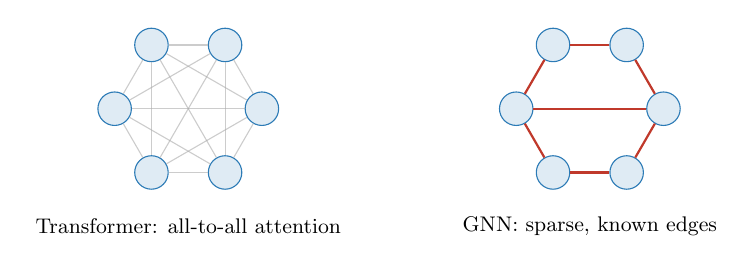
\begin{tikzpicture}[scale=0.85, every node/.style={transform shape},
      n/.style={circle, draw=acc2, fill=acc2!15, minimum size=5mm, inner sep=0pt}]
      \begin{scope}
        \foreach \i in {0,...,5} \node[n] (a\i) at (\i*60:1.1) {};
        \foreach \i/\j in {0/1,0/2,0/3,0/4,0/5,1/2,1/3,1/4,1/5,
                           2/3,2/4,2/5,3/4,3/5,4/5}
          \draw[dim, opacity=0.6] (a\i)--(a\j);
        \node at (0,-1.75) {\small Transformer: all-to-all attention};
      \end{scope}
      \begin{scope}[xshift=6cm]
        \foreach \i in {0,...,5} \node[n] (b\i) at (\i*60:1.1) {};
        \foreach \i/\j in {0/1,1/2,2/3,3/4,4/5,5/0,0/3}
          \draw[acc, thick] (b\i)--(b\j);
        \node at (0,-1.75) {\small GNN: sparse, known edges};
      \end{scope}
    \end{tikzpicture}
  \end{center}
  \vspace{0.3em}
  \begin{itemize}\small
    \item Self-attention sends a message $m_{ij} = \mathrm{softmax}_j(q_i
          \cdot k_j / \sqrt{d})\, W_v h_j$ from every token $j$ to every
          token $i$. That is MSG + AGG on the complete graph.
    \item GAT restricts the same computation to real edges, with additive
          instead of dot-product attention.
    \item The equivalence breaks at three points: \alert{positional encodings}
          (without them, the Transformer treats its input as a set),
          the \alert{feed-forward block} (per-node, no graph analogue),
          and \alert{LayerNorm / residual stream}.
  \end{itemize}
\end{frame}
\note{Ask the smartest question in the room before anyone else does. This removes
the objection that otherwise stays with a listener for 20 minutes.

The mapping (Joshi 2020/2025, Dwivedi \& Bresson 2021): nodes = tokens,
edges = all-to-all, MSG = value vector scaled by softmax attention, AGG = sum.
GAT is the sparse case. The FFN, residual, and LayerNorm are non-graph parts.

CHECKPOINT: 17:28 by the end of this slide. Movement 3 starts now.}

% -------------------------------------------------------------------------
\begin{frame}{Sparse known graph vs.\ learned attention: a decision rule}
  \vspace{0.1em}
  \begin{center}
    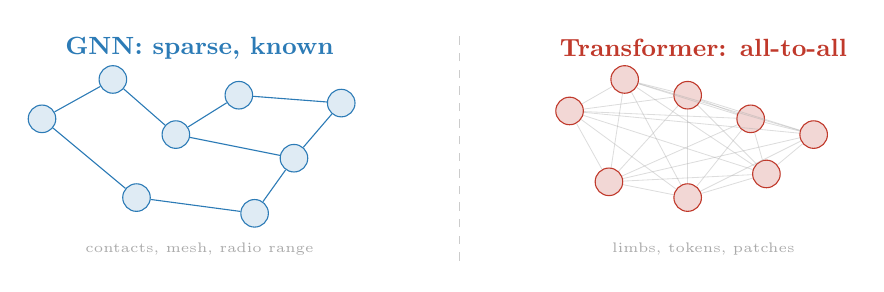
\begin{tikzpicture}[
      font=\scriptsize,
      nd/.style={circle, draw=acc2, fill=acc2!15, minimum size=3.5mm,
                 inner sep=0pt},
      hl/.style={circle, draw=acc, fill=acc!20, minimum size=3.5mm,
                 inner sep=0pt},
      ed/.style={acc2, line width=0.4pt},
      eda/.style={dim, line width=0.3pt, opacity=0.4},
    ]
    % Left: sparse known graph (GNN wins)
    \node[font=\small\bfseries, acc2] at (1.8, 2.4) {GNN: sparse, known};
    \foreach \i/\x/\y in {0/-0.2/1.5, 1/0.7/2.0, 2/1.5/1.3, 3/2.3/1.8,
                           4/3.0/1.0, 5/3.6/1.7, 6/1.0/0.5, 7/2.5/0.3}
      \node[nd] (L\i) at (\x,\y) {};
    \draw[ed] (L0)--(L1); \draw[ed] (L1)--(L2); \draw[ed] (L2)--(L3);
    \draw[ed] (L3)--(L5); \draw[ed] (L2)--(L4); \draw[ed] (L4)--(L5);
    \draw[ed] (L0)--(L6); \draw[ed] (L6)--(L7); \draw[ed] (L4)--(L7);
    \node[font=\tiny, color=dim, align=center] at (1.8, -0.15)
      {contacts, mesh, radio range};

    % Right: complete graph (Transformer wins)
    \node[font=\small\bfseries, acc] at (8.2, 2.4) {Transformer: all-to-all};
    \foreach \i/\x/\y in {0/6.5/1.6, 1/7.2/2.0, 2/8.0/1.8, 3/8.8/1.5,
                           4/7.0/0.7, 5/8.0/0.5, 6/9.0/0.8, 7/9.6/1.3}
      \node[hl] (R\i) at (\x,\y) {};
    \foreach \i in {0,...,7} {
      \foreach \j in {\i,...,7} {
        \ifnum\i<\j \draw[eda] (R\i)--(R\j); \fi
      }
    }
    \node[font=\tiny, color=dim, align=center] at (8.2, -0.15)
      {limbs, tokens, patches};

    % divider
    \draw[black!20, dashed] (5.1, -0.3) -- (5.1, 2.6);
    \end{tikzpicture}
  \end{center}
  \vspace{-0.1em}
  \begin{columns}[T]
    \begin{column}{0.47\textwidth}
      \small
      GNS generalizes to $10\times$ more particles.
      RoboBallet generalizes zero-shot to new placements.
      Li \& Prorok's planner scales to larger teams.
      \vspace{0.2em}

      {\scriptsize\color{dim}\arx{2002.09405}\ \arx{2509.05397}\ \arx{1912.06095}}
    \end{column}
    \begin{column}{0.47\textwidth}
      \small
      Amorpheus (ICLR 2021): encoding the kinematic tree
      \alert{hurt} morphology control. Point Transformer v3 (CVPR 2024)
      displaced DGCNN on point clouds.
      \vspace{0.2em}

      {\scriptsize\color{dim}\arx{2106.03672}\ \arx{2408.16932}}
    \end{column}
  \end{columns}
\end{frame}
\note{The two diagrams show the structural assumption side by side.
Left: a sparse graph where each node connects to a few physical neighbors.
Right: a complete graph where attention learns which connections matter.

The decision rule: encode the sparse graph when the edges are physical, cheap
to compute, and you need size generalization with limited data. Learn the edges
when the graph is an artifact or data is abundant.}


% =========================================================================
% Close
% =========================================================================

% --- 13 ---------------------------------------------------------------
\begin{frame}{When a Transformer outperforms a GNN}
  \vspace{0.6em}
  \begin{itemize}
    \setlength{\itemsep}{0.6em}
    \item \textbf{Small and dense graph}: a Transformer computes the same thing
      on a complete graph, and the tooling is better.
    \item \textbf{Invented edges}: Kurin et al.\ (ICLR 2021) showed that
      encoding the kinematic tree \alert{hurt} morphology control.
    \item \textbf{Grid or sequence}: a CNN or Transformer already encodes
      that structure.
    \item \textbf{Abundant data}: RT-1/2, Octo, OpenVLA and $\pi_0$ learn
      edges from scratch as Transformer-native VLA policies.
  \end{itemize}
  \vfill
  \begin{center}\large
    A GNN outperforms a Transformer when the \alert{interaction graph is
    sparse, physically real, and the data is limited}.
  \end{center}
\end{frame}
\note{The Amorpheus result (Kurin et al.\ 2021) is the counterexample that
teaches judgment: the physical graph existed and hurt. Point Transformer v3
displaced DGCNN on point clouds. The whole VLA stack is Transformer-native.

But RoboBallet (Science Robotics 2025), the learned-simulator line (GNS,
MeshGraphNets), and multi-robot coordination (Li \& Prorok) all held with
GNNs. The field has converged on hybrids (GraphGPS), but T\"onshoff et al.\
(LoG 2023) showed that tuned MPNNs close most of the reported gap.}

% --- 14 ---------------------------------------------------------------
\begin{frame}{Three-question test for graph-structured problems}
  \vspace{1.2em}
  \begin{enumerate}
    \setlength{\itemsep}{1.3em}
    \item \Large Do I have \alert{entities with relations} between them?
    \item \Large Is there \alert{no natural ordering} of those entities?
    \item \Large Does the \alert{number of them change}?
  \end{enumerate}
  \vspace{1.4em}
  \begin{center}\large
    \textbf{Two yeses} $\Rightarrow$ a GNN is worth testing.
  \end{center}
\end{frame}
\note{Slow down. The whole talk exists so they can recognize when their own
problem is a graph.

Give them five seconds of silence to test their own project against it.}

% --- 15 ---------------------------------------------------------------
\begin{frame}{Take-home}
  \vspace{0.2em}
  \begin{center}
    \large
    A GNN repeats one operation: \alert{each node aggregates its neighbors,
    then updates its own vector.}\\[0.6em]
    \alert{Graph construction} decides performance.
  \end{center}
  \vspace{0.6em}
  \hrule
  \vspace{0.4em}
  \scriptsize
  \textbf{Five papers to read, in order}
  \begin{itemize}\setlength{\itemsep}{0.05em}
    \item Joshi, ``Transformers are Graph Neural Networks'' (2020/2025)
    \item Sanchez-Gonzalez et al., GNS (ICML 2020) \arx{2002.09405}
    \item Kurin et al., Amorpheus (ICLR 2021) \arx{2106.03672}
    \item Ramp\'{a}\v{s}ek et al., GraphGPS (NeurIPS 2022) \arx{2205.12454}
    \item T\"{o}nshoff et al., ``Where Did the Gap Go?'' (LoG 2023) \arx{2309.00367}
  \end{itemize}
\end{frame}
\note{Say the one-thing sentence one last time, word for word as on slide 2. Then give the resources, fast.

CHECKPOINT: 17:48. You promised 17:50. Finish early.}

% --- 16 ---------------------------------------------------------------
\begin{frame}[plain]
  \vspace{2.2em}
  \begin{center}
    {\Huge Questions?}\\[2.0em]
    {\large\color{dim}
      \CJK{仲翊} \quad$\cdot$\quad MiRA Training Course 2026}\\[0.8em]
    {\small\color{dim}
      Slides and notebooks:
      \texttt{github.com/Chung-I/MiRA\_training\_course\_2026}}
  \end{center}
\end{frame}
\note{Q\&A prep:

* "Isn't a Transformer just a GNN?" -> Yes: self-attention is message passing
  on the complete graph, where the message is a value vector scaled by softmax
  attention. GAT is the same computation restricted to real edges. The
  equivalence breaks at positional encodings (without them, a Transformer treats
  its input as a set), the per-token FFN (no graph analogue), and LayerNorm.
  (Joshi 2020/2025, Dwivedi \& Bresson 2021.)

* "How many layers?" -> Start at 2. Over-smoothing collapses representations
  at 4--6 layers. Over-squashing (Alon \& Yahav 2021) is a separate problem:
  information from an exponentially growing receptive field compresses into a
  fixed-size vector. Di Giovanni et al.\ (ICML 2023) proved that depth does
  not fix it --- widen the network, or add a global node, or rewire.

* "How do I build the graph for a point cloud?" -> k-NN with k around 16--20
  in xyz, edge feature = relative position. DGCNN recomputes edges in feature
  space each layer. Point Transformer v3 (CVPR 2024) now leads on S3DIS and
  SemanticKITTI by replacing the k-NN graph with full attention over points.

* "Are GNNs still relevant?" -> RoboBallet (Science Robotics 2025) and the
  learned-simulator line (GNS, MeshGraphNets) are active. A known sparse
  graph wins on sample efficiency and size generalization. But Amorpheus
  (ICLR 2021) showed the kinematic tree hurts morphology control, and VLA
  policies (RT-1/2, Octo, OpenVLA, pi0) are Transformer-native. The field
  has converged on hybrids (GraphGPS: local MPNN + global attention + PE).
  T\"onshoff et al.\ (LoG 2023) showed that tuned MPNNs close most of the
  reported graph-transformer gap on long-range benchmarks.

* "Which library?" -> PyTorch Geometric (PyG). DGL if you need heterogeneous
  graphs. The four official PyG Colab tutorials are on the previous slide.

* "What about expressiveness / WL?" -> One sentence: MPNNs are bounded by
  1-WL (Xu et al.\ 2019). Graph transformers with the right positional
  encodings exceed 1-WL and reach between 1-WL and 3-WL (TokenGT, Graphormer,
  GRIT). But higher WL expressiveness does not reliably predict benchmark
  accuracy. Give the sentence and move on.}

% =========================================================================
\appendix
% =========================================================================

\begin{frame}{Backup: over-smoothing vs.\ training difficulty on Cora}
  \vspace{-0.2em}
  \centering\scriptsize
  \textbf{GCN on Cora}, hidden=16, 5 seeds. Train/test accuracy and mean
  pairwise cosine distance between node embeddings.
  \vspace{0.2em}

  \begin{tabular}{@{}rrrrrr@{}}
    \toprule
    & \multicolumn{2}{c}{\textbf{baseline}} &
      \multicolumn{2}{c}{\textbf{+\,residual}} & \\
    \cmidrule(lr){2-3}\cmidrule(lr){4-5}
    \textbf{layers} & train & test & train & test & \textbf{dist (base)} \\
    \midrule
    2 & 100.0 & \textcolor{good}{\textbf{80.8}} & 100.0 & 80.8 & 0.234 \\
    4 & 100.0 & 77.6 & 100.0 & 79.7 & 0.266 \\
    6 & 100.0 & 73.1 & 100.0 & \textcolor{good}{78.5} & 0.278 \\
    8 & \textcolor{acc}{\textbf{82.4}} & \textcolor{acc}{\textbf{53.8}}
      & 100.0 & 74.6 & 0.322 \\
    \bottomrule
  \end{tabular}
  \vspace{0.4em}

  \small
  \begin{columns}[T]
    \begin{column}{0.47\textwidth}
      \textbf{2--6 layers:} all variants reach 100\% train accuracy.
      The test accuracy drop (80.8\% $\rightarrow$ 73.1\%) comes from
      \alert{over-smoothing}: embeddings become less discriminative, and the
      model generalizes worse despite fitting the training set.
    \end{column}
    \begin{column}{0.47\textwidth}
      \textbf{8 layers:} the baseline train accuracy drops to 82.4\%.
      \alert{Residual connections} fix this to 100\%, confirming training
      difficulty (vanishing gradients). But test accuracy still drops to
      74.6\%, because over-smoothing degrades generalization even when
      training succeeds.
    \end{column}
  \end{columns}
\end{frame}
\note{Backup. The ablation is in Section 6 of
\texttt{notebooks/pyg\_node\_classification.ipynb}. Open it in Colab to see
the cached outputs.

The key finding: residuals fix the training failure at 8 layers (82.4\%
$\rightarrow$ 100\% train) but do not fix the test accuracy loss (74.6\% test,
down from 80.8\% at 2 layers). Over-smoothing degrades generalization even
when training succeeds. Both factors contribute at different depths.

Li et al., ``Deeper Insights into Graph Convolutional Networks for
Semi-Supervised Learning,'' AAAI 2018.}

\end{document}
